\subsubsection{2-Tore} \label{subsubsec:2tore}

In der Elektrotechnik sind 2-Tore, Systeme mit 2 Klemmenpaaren (Tore). 
Diese sind intern aus beliebigen R (ohmischer Widerstand), L (Induktivität), C (Kapazität) und M(Gegeninduktivität) Komponenten aufgebaut. 
Dabei wird ein Tor als Eingang für ein Elektrisches Signal verwendet. Folglich wird bei den Ausgangsklemmen das Ausgangssignal abgegriffen. 
Es wird zwischen aktiv und passiv unterschieden.
Bei aktiven Zweitoren wird die Leistung, die beim Eingang eingespeist wird, verstärkt. 
Im Vergleich dazu wird beim passiven die Leistung am Ausgang kleiner.

\begin{figure}[H]
	\centering
	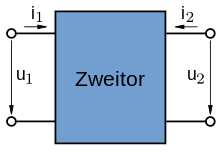
\includegraphics[width=5cm]{2Tor.png}
	\label{fig:übersicht}
\end{figure}